\chapter{From Particles to a Simple Quantum Field}

These notes follow Leonard Susskind's seventh lecture in \emph{Advanced Quantum Mechanics}. The lecture is deliberately a second pass through the construction of a simple quantum field: not quite a repetition, but the same idea rebuilt more slowly and from a slightly different angle. Susskind starts from particles, not from classical fields, and asks what formalism can describe one particle, two particles, or any number of particles, including situations in which the number changes. The answer is a nonrelativistic field theory for a single species of particle. The exposition below keeps that order, that pacing, and that motivation, with curation by LazyingArt LLC.

\section{Why One Needs Fields}

Susskind opens by reminding the audience that there are two routes into the subject. One can begin with particles and understand why they are naturally described by fields, or one can begin with fields and understand why wave fields come in quanta. This lecture stays with the first route.

The motivation is physical before it is formal. Fixed-particle-number quantum mechanics is perfectly adequate if one insists on studying one particle, or two particles, or any other predetermined number. But the world does not work that way. Photons are emitted and absorbed continually. Unstable particles decay. A neutron can decay into a proton, an electron, and a neutrino, and in the process the particle content changes. If quantum mechanics is to accommodate such processes within a single framework, it must allow the number of particles to vary.

The lecture therefore narrows the scope in order to sharpen the idea. There is one species of nonrelativistic particle, and one wants a formalism broad enough to describe all occupation numbers of that species at once. Susskind also warns at the outset that the mathematics is not hard, but it is abstract; this is why he restarts the construction from the one-particle theory and rebuilds the necessary pieces carefully.

\section{Single-Particle Quantum Mechanics Recalled}

The starting point is ordinary one-particle quantum mechanics. If $|\psi\rangle$ is the state of a single particle and $|x\rangle$ denotes a state localized at position $x$, then the wavefunction is
\begin{equation}
\psi(x)=\langle x|\psi\rangle.
\end{equation}
This is a probability amplitude. The corresponding probability density is
\begin{equation}
|\psi(x)|^2=\psi^*(x)\psi(x),
\end{equation}
and for a normalized one-particle state,
\begin{equation}
\int dx\,\psi^*(x)\psi(x)=1.
\end{equation}

Susskind is careful here about notation. Lower-case $\psi$ refers to an ordinary one-particle wavefunction. It is not yet a field, not yet an operator, and not yet an object living in the many-particle Hilbert space. That distinction is one of the recurring lessons of the lecture.

There is also a useful small observation at this stage. In the one-particle problem, the integral of $|\psi(x)|^2$ is the total probability, hence $1$. Since there is exactly one particle in the problem, it also happens, trivially, to be the total number of particles. Later the same-looking integral will reappear with a nontrivial meaning.

\section{Modes, Orthogonality, and the Delta Function}

Next Susskind chooses a convenient basis of one-particle states. There are many choices: the position eigenstates themselves form a basis, as do the eigenstates of any Hermitian operator. For the later construction, energy eigenstates are especially natural.

His concrete example is a particle in a box. The horizontal axis represents position, the vertical axis the potential energy, and the potential rises steeply at the walls. The first few energy eigenfunctions are essentially sine waves, ordered by their nodes.

\begin{figure}[t]
\centering
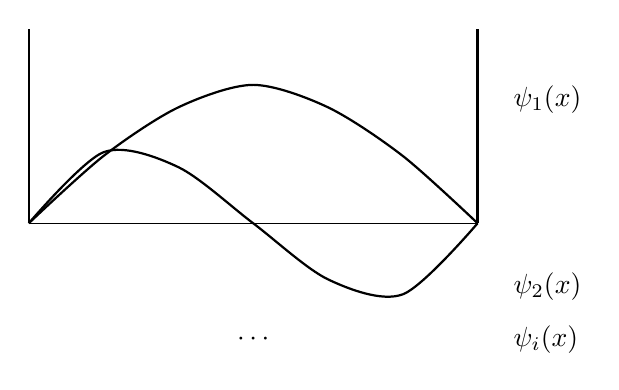
\begin{tikzpicture}[scale=0.95]
\draw[thick] (0,0) -- (0,2.6);
\draw[thick] (6,0) -- (6,2.6);
\draw[thin] (0,0) -- (6,0);

\draw[thick, smooth] plot coordinates {(0,0) (1,0.9) (2,1.55) (3,1.85) (4,1.55) (5,0.9) (6,0)};
\draw[thick, smooth] plot coordinates {(0,0) (1,0.95) (2,0.75) (3,0) (4,-0.75) (5,-0.95) (6,0)};

\node[right] at (6.35,1.65) {$\psi_1(x)$};
\node[right] at (6.35,-0.85) {$\psi_2(x)$};
\node[right] at (6.35,-1.55) {$\psi_i(x)$};
\node at (3,-1.55) {$\cdots$};
\end{tikzpicture}
\caption{A clean schematic of the particle-in-a-box modes drawn in the spirit of the lecture board: the first few sine-like eigenfunctions, organized by node count, with labels matching Susskind's notation.}
\end{figure}

If the one-particle eigenfunctions are written $\psi_i(x)$, then orthonormality means
\begin{equation}
\int dx\,\psi_i^*(x)\psi_j(x)=\delta_{ij}.
\end{equation}
Completeness means that the corresponding one-particle states satisfy
\begin{equation}
\sum_i |i\rangle\langle i|=\mathbf{1}.
\end{equation}

This is the point at which Susskind inserts what he calls a little trick, one that recurs all through the subject. Sandwich the identity operator between position states:
\begin{align}
\langle x|y\rangle
&=\langle x|\mathbf{1}|y\rangle \\
&=\sum_i \langle x|i\rangle\langle i|y\rangle \\
&=\sum_i \psi_i(x)\psi_i^*(y).
\end{align}
Since $\langle x|y\rangle=\delta(x-y)$, one obtains the position-space completeness relation
\begin{equation}
\sum_i \psi_i(x)\psi_i^*(y)=\delta(x-y).
\end{equation}
The placement of the complex conjugation depends on the bra-ket order, but this is the convention used here and it will be kept fixed throughout.

This identity is the last major one-particle ingredient needed later. In Susskind's phrase, this is the basic mathematics.

\section{From Occupation Numbers to the Field Operator}

Only after the one-particle scaffold is in place does the lecture return to the many-particle problem. The Hilbert space now changes. Instead of one-particle wavefunctions, one uses occupation-number states
\begin{equation}
|n_1,n_2,\ldots\rangle,
\end{equation}
where $n_i$ is the number of particles occupying the one-particle mode $i$. These states belong to Fock space; they do not lie in the same vector space as the one-particle functions $\psi_i(x)$.

To change occupation numbers one introduces, for each mode $i$, a creation operator and an annihilation operator,
\begin{equation}
a_i^\dagger,\qquad a_i.
\end{equation}
The operator $a_i^\dagger$ creates a particle in mode $i$, while $a_i$ annihilates one. The associated number operator is
\begin{equation}
N_i=a_i^\dagger a_i.
\end{equation}
The vacuum is the state with all occupation numbers zero,
\begin{equation}
|0\rangle = |0,0,\ldots\rangle.
\end{equation}
A one-particle state occupying the mode $i$ is therefore
\begin{equation}
|i\rangle=a_i^\dagger|0\rangle.
\end{equation}

At first this oscillator language is only bookkeeping. Susskind says so explicitly. It will become more than bookkeeping later, but the immediate purpose is simply to create a formalism in which occupation numbers can be raised and lowered systematically.

Now comes the key definition:
\begin{equation}
\Psi(x)=\sum_i a_i\,\psi_i(x),
\qquad
\Psi^\dagger(x)=\sum_i a_i^\dagger\,\psi_i^*(x).
\end{equation}
These are operator-valued functions of position: at each point $x$ there is an operator. The notation is deliberately similar to the one-particle wavefunction, but the object is completely different. $\Psi(x)$ is not a one-particle state. It is an operator acting on Fock space.

The analogy with Fourier expansion is direct. If the basis functions $\psi_i(x)$ were plane waves, then the coefficients of the expansion would be the Fourier coefficients. The only novelty is that here the coefficients are not ordinary numbers but operators.

This is exactly where Susskind distinguishes c-numbers from q-numbers. The wavefunctions $\psi_i(x)$ are ordinary complex numbers as functions of $x$; they commute with everything. The $a_i$ and $a_i^\dagger$ are operators. Because the wavefunctions are c-numbers, one may move them freely through the expressions without any operator-ordering issue.

Neither $\Psi(x)$ nor $\Psi^\dagger(x)$ is Hermitian. Their adjoints are each other. But the combinations
\begin{equation}
\Psi(x)+\Psi^\dagger(x),
\qquad
i\bigl(\Psi^\dagger(x)-\Psi(x)\bigr)
\end{equation}
are Hermitian, hence observable. Susskind mentions this not to begin a measurement theory of $\Psi$ immediately, but to show that field-like observables do emerge from these operator-valued functions.

The most useful way to motivate the definition is to ask what it does. Insert the resolution of the identity into the position state:
\begin{align}
|x\rangle
&=\mathbf{1}|x\rangle \\
&=\sum_i |i\rangle\langle i|x\rangle \\
&=\sum_i a_i^\dagger|0\rangle\,\psi_i^*(x) \\
&=\Psi^\dagger(x)|0\rangle.
\end{align}
Thus $\Psi^\dagger(x)$ creates, out of the vacuum, a particle localized at the point $x$. This is the intuitive content of the field operator. The operators $a_i^\dagger$ create particles in definite modes; the operator $\Psi^\dagger(x)$ creates a particle at a definite position.

\section{Playing with the Field: Number and Density}

At this point Susskind does not yet write a field equation. Instead he plays with the field and asks what simple observables can be built from it. The first one is
\begin{equation}
\int dx\,\Psi^\dagger(x)\Psi(x).
\end{equation}
This resembles the one-particle normalization integral, but the resemblance is only formal. Here $\Psi$ and $\Psi^\dagger$ are operators.

Substituting the definitions gives
\begin{align}
\int dx\,\Psi^\dagger(x)\Psi(x)
&=\int dx
\left(\sum_i a_i^\dagger\psi_i^*(x)\right)
\left(\sum_j a_j\psi_j(x)\right) \\
&=\int dx\,\sum_{i,j} a_i^\dagger a_j\,\psi_i^*(x)\psi_j(x) \\
&=\sum_{i,j} a_i^\dagger a_j \int dx\,\psi_i^*(x)\psi_j(x) \\
&=\sum_{i,j} a_i^\dagger a_j\,\delta_{ij} \\
&=\sum_i a_i^\dagger a_i.
\end{align}
Therefore
\begin{equation}
N=\int dx\,\Psi^\dagger(x)\Psi(x)=\sum_i a_i^\dagger a_i=\sum_i N_i
\end{equation}
is the total-number operator.

This is the first major payoff of the field construction. The same formal structure that, in one-particle quantum mechanics, integrated to total probability, now integrates to the total number of particles in the many-particle system.

It is then natural to interpret the integrand itself as a local density:
\begin{equation}
n(x)=\Psi^\dagger(x)\Psi(x).
\end{equation}
If one integrates this over a small spatial region $R$, one obtains
\begin{equation}
N_R=\int_R dx\,n(x),
\end{equation}
the operator that counts how many particles lie in that region.

Here Susskind slows down again, because the temptation is strong to call $n(x)$ a probability density. He does not want to make that identification too quickly. In a many-particle state, what one measures in a small region is the number of particles in that region. If there are many particles, dividing by the total number often gives something that tracks a probability distribution extremely well in practice, but it is not \emph{identically} the one-particle Born-rule density. The many-particle operator $n(x)$ is an observable, with fluctuations from state to state and measurement to measurement. It is safest to call it what it is: the particle-density operator.

\section{A Slightly Different Thing: Energy}

Having stabilized the particle-counting story, Susskind says that he wants to do a slightly different thing. The new target is the total energy.

He first restricts the discussion to independent particles, meaning particles that do not interact with one another. This is an approximation, but often a good one for dilute systems. In that approximation the total energy is the sum over modes of occupation number times one-particle energy:
\begin{equation}
H=\sum_i \omega_i a_i^\dagger a_i.
\end{equation}
Here $\omega_i$ is simply the energy of the $i$th one-particle mode. Susskind keeps the symbol $\omega_i$ from the oscillator language, while also saying explicitly that it is the energy.

To understand these $\omega_i$, he returns to the one-particle time-independent Schr\"odinger equation. From here on we set $\hbar=1$. On the board he writes
\begin{equation}
\left[\frac{P^2}{2m}+V(x)\right]\psi_i(x)=\omega_i\psi_i(x),
\qquad
P=-i\,\frac{\partial}{\partial x}.
\end{equation}
For cleaner notation in the rest of the chapter, let us write the one-particle momentum operator as
\begin{equation}
p=-i\,\partial_x,
\end{equation}
and reserve the symbol $P$ for the total momentum operator of the field. Then the one-particle equation is
\begin{equation}
\left[\frac{p^2}{2m}+V(x)\right]\psi_i(x)=\omega_i\psi_i(x).
\end{equation}
In three-dimensional language this becomes
\begin{equation}
\left[-\frac{\nabla^2}{2m}+V(x)\right]\psi_i(x)=\omega_i\psi_i(x).
\end{equation}

Susskind does not solve this equation in the lecture. He uses it instead as an identity that can be inserted into the many-particle calculation. Before making the jump, he recalls one more familiar one-particle formula:
\begin{equation}
\int dx\,\psi^*(x)\left(-\frac{\nabla^2}{2m}+V(x)\right)\psi(x),
\end{equation}
which is the expectation value of the energy in the one-particle state $\psi$.

Now comes the same leap that worked for particle number. Replace the little $\psi$ by the big $\Psi$. The guess is that the Hamiltonian operator can be written as
\begin{equation}
H=\int dx\,\Psi^\dagger(x)\left(-\frac{\nabla^2}{2m}+V(x)\right)\Psi(x).
\end{equation}
This is exactly the form suggested by the lecture board. Susskind writes the answer first and then proves that it is equal to the mode sum. He also continues to write $\int dx$ even after promoting the kinetic term to $-\nabla^2/2m$; the important point here is the local operator density, not the measure notation.

Expand the field operators:
\begin{align}
H
&=\int dx
\left(\sum_i a_i^\dagger\psi_i^*(x)\right)
\left(-\frac{\nabla^2}{2m}+V(x)\right)
\left(\sum_j a_j\psi_j(x)\right) \\
&=\sum_{i,j} a_i^\dagger a_j
\int dx\,\psi_i^*(x)\left(-\frac{\nabla^2}{2m}+V(x)\right)\psi_j(x).
\end{align}
At this point the one-particle Schr\"odinger equation is used:
\begin{equation}
\left(-\frac{\nabla^2}{2m}+V(x)\right)\psi_j(x)=\omega_j\psi_j(x).
\end{equation}
Therefore
\begin{align}
H
&=\sum_{i,j} a_i^\dagger a_j
\int dx\,\psi_i^*(x)\,\omega_j\psi_j(x) \\
&=\sum_{i,j} a_i^\dagger a_j\,\omega_j
\int dx\,\psi_i^*(x)\psi_j(x) \\
&=\sum_{i,j} a_i^\dagger a_j\,\omega_j\,\delta_{ij} \\
&=\sum_j \omega_j a_j^\dagger a_j,
\end{align}
which is exactly the original expression for the total energy.

This calculation also clarifies an operator-ordering point that comes up in the lecture discussion. Nothing here required commuting an annihilation operator past a creation operator. The wavefunctions $\psi_i(x)$ are c-numbers, so they may be moved freely. The derivatives act on the ordinary wavefunctions, not on the operators $a_i$ and $a_i^\dagger$.

Susskind writes this object on the board as the energy, but at the same time insists that it is an operator. In modern language one would simply say that it is the Hamiltonian operator, hence also the total-energy operator:
\begin{equation}
H=\int dx\,\mathcal{H}(x),
\qquad
\mathcal{H}(x)=\Psi^\dagger(x)\left(-\frac{\nabla^2}{2m}+V(x)\right)\Psi(x).
\end{equation}
The integrand is naturally called the energy density. Susskind adds one cautionary sentence: this is a definition of the local energy density for the present Hamiltonian, not a mathematically unique notion in every context.

\section{Why This Is a Field and What Comes Next}

At this point the audience asks the natural question: why should this be called a field at all? Susskind's answer is direct. It is a quantity that depends on position, and suitable Hermitian combinations of it are observable. One can speak of it at one point of space and at another. It produces a local particle density and a local energy density. In that mathematical and physical sense, it is a field.

It is not, however, the electromagnetic field. The lecture keeps the discussion nonrelativistic. As long as the particles are slow enough that the one-particle energy is of the form $p^2/2m$ plus a potential, this is the field whose quanta are those particles. Protons, neutrons, or electrons moving slowly would all fit this pattern. The particles are the quanta of the field in exactly the same structural sense that photons are the quanta of the electromagnetic field.

The formalism also contains ordinary one-particle quantum mechanics as a special case. If one restricts to the sector in which the total number operator has eigenvalue $1$, the whole construction collapses back to the usual one-particle theory. In that sense nothing has been abandoned; the Hilbert space has simply been enlarged.

At the opposite extreme, states with very large occupation number begin to behave classically. Susskind emphasizes that expectation values then follow the same sort of equations of motion as the corresponding classical fields. For the present nonrelativistic system, the expectation value of the field operator satisfies, in essence, the time-dependent Schr\"odinger equation:
\begin{equation}
i\,\partial_t\langle\Psi(x,t)\rangle
=
\left(-\frac{\nabla^2}{2m}+V(x)\right)\langle\Psi(x,t)\rangle.
\end{equation}
This statement is asserted rather than derived in detail in the lecture, but it is the crucial link between the quantum field and its classical limit.

A late aside in the lecture looks ahead to relativity. There Susskind warns that particle position is not the best concept, and therefore particle density is not generally the right observable. Energy density is much better behaved. He mentions, only heuristically, that for electromagnetic radiation quantities such as $E^2+B^2$ play the role of energy density. This aside is useful as intuition, but it lies outside the main nonrelativistic derivation.

The final step of the lecture is another preview. For a one-particle wavefunction,
\begin{equation}
\langle p\rangle_\psi
=
\int dx\,\psi^*(x)\left(-i\,\partial_x\right)\psi(x).
\end{equation}
By the same replacement rule that carried probability density to number density, and one-particle energy to field Hamiltonian, one is led to the total momentum operator of the field:
\begin{equation}
P=\int dx\,\Psi^\dagger(x)\left(-i\,\partial_x\right)\Psi(x).
\end{equation}
Susskind does not fully derive this in the lecture. He presents it as the next natural observable and a teaser for the next meeting, stressing that it is an operator, not an expectation value. An operator and a state together produce an expectation value; the operator alone is the observable itself.

\section{Summary}

The lecture reconstructs a simple quantum field from the particle side. The motivation is the need to describe arbitrary and changing particle number. The construction begins with ordinary one-particle wavefunctions, orthonormal modes, and the completeness relation, then passes to Fock space, where occupation numbers are changed by creation and annihilation operators. Out of these ingredients one defines the field operators $\Psi(x)$ and $\Psi^\dagger(x)$, interprets $\Psi^\dagger(x)$ as creating a particle at the point $x$, derives the total-number operator and the particle-density operator, and finally rewrites the mode-sum energy as the Hamiltonian
\begin{equation}
H=\int dx\,\Psi^\dagger(x)\left(-\frac{\nabla^2}{2m}+V(x)\right)\Psi(x).
\end{equation}
That is the lecture's central payoff: the many-particle system can be described as a field whose quanta are the particles themselves. The next step, deferred to the following lecture, is to use these field operators to represent actual processes such as scattering and decay.